% Standalone vector figure extracted from manuscript.tex.
% Rebuild all figures from the project root: bash tkz/build.sh
\documentclass[tikz,border=2pt,class=IEEEtran]{standalone}
\usepackage{amsmath,amssymb,amsfonts}
\usepackage{xcolor}
\usetikzlibrary{positioning,arrows.meta,calc,backgrounds}

% Match the manuscript's IEEE Access text and math font settings.
\renewcommand{\textbf}[1]{{\fontseries{b}\selectfont #1}}
\renewcommand{\textit}[1]{{\itshape #1}}
\makeatletter
\AtBeginDocument{%
  \fontencoding{T1}\rmfamily\fontseries{m}\fontsize{10}{12}\selectfont
  \gdef\operator@encoding{T1}%
  \gdef\encodingdefault{T1}}
\makeatother

% ---- shared palette for review figures ----
\definecolor{cVLA}{HTML}{34618E}   % VLA lane / policy blue
\definecolor{cWM}{HTML}{9E4A3F}    % world-model lane
\definecolor{cCONV}{HTML}{5E4B8B}  % convergence purple
\definecolor{cGood}{HTML}{3A7D44}  % verified green
\definecolor{cWarn}{HTML}{B07A2A}  % caution amber
\definecolor{cPale}{HTML}{F2F0EA}  % pale panel fill
\tikzset{
  fnode/.style={draw=black!55, fill=white, rounded corners=1.5pt,
                inner sep=2.5pt, align=center, font=\fontsize{8}{9.5}\selectfont},
  flane/.style={draw=none, rounded corners=2pt, inner sep=3pt,
                align=center, font=\fontsize{8}{9.5}\selectfont\bfseries, text=white},
  farr/.style={-{Stealth[length=2mm]}, thick, black!60},
}


\newcommand{\figfont}{\fontsize{8}{9.5}\selectfont}

\begin{document}

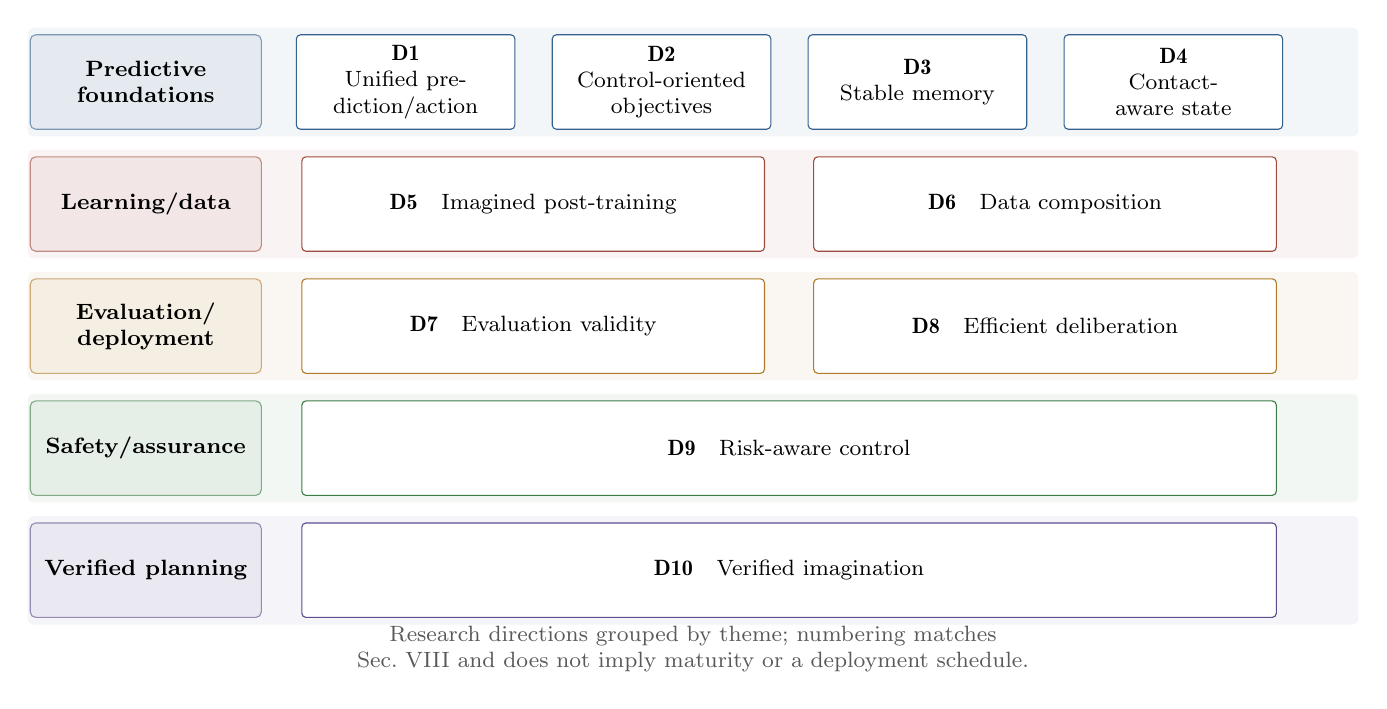
\begin{tikzpicture}[font=\figfont]
\tikzset{theme/.style={fill=#1!13,draw=#1!65,rounded corners=2pt,text width=27mm,minimum height=12mm,align=center,font=\figfont\bfseries},
 item/.style={fnode,text width=#1,minimum height=12mm}}
\foreach \y/\bandcolor/\label in {
 0/cVLA/{Predictive foundations},
 -1.55/cWM/{Learning/data},
 -3.10/cWarn/{Evaluation/\\deployment},
 -4.65/cGood/{Safety/assurance},
 -6.20/cCONV/{Verified planning}}{
 \fill[\bandcolor!6,rounded corners=2pt] (0,\y-.69) rectangle (16.9,\y+.69);
 \node[theme=\bandcolor] at (1.5,\y) {\label};}
\node[item=26mm,draw=cVLA] at (4.8,0) {\textbf{D1}\\Unified prediction/action};
\node[item=26mm,draw=cVLA] at (8.05,0) {\textbf{D2}\\Control-oriented objectives};
\node[item=26mm,draw=cVLA] at (11.3,0) {\textbf{D3}\\Stable memory};
\node[item=26mm,draw=cVLA] at (14.55,0) {\textbf{D4}\\Contact-aware state};
\node[item=57mm,draw=cWM] at (6.42,-1.55) {\textbf{D5}\quad Imagined post-training};
\node[item=57mm,draw=cWM] at (12.92,-1.55) {\textbf{D6}\quad Data composition};
\node[item=57mm,draw=cWarn] at (6.42,-3.10) {\textbf{D7}\quad Evaluation validity};
\node[item=57mm,draw=cWarn] at (12.92,-3.10) {\textbf{D8}\quad Efficient deliberation};
\node[item=122mm,draw=cGood] at (9.67,-4.65) {\textbf{D9}\quad Risk-aware control};
\node[item=122mm,draw=cCONV] at (9.67,-6.20) {\textbf{D10}\quad Verified imagination};
\node[black!65,align=center,text width=159mm] at (8.45,-7.2)
 {Research directions grouped by theme; numbering matches Sec.~VIII and does not imply maturity or a deployment schedule.};
\end{tikzpicture}
\end{document}
